\documentclass[a4paper]{jpconf}
\usepackage{amssymb,amsfonts,amsmath,mathtext,mathtools}
\usepackage{xfrac}
\usepackage{url, hyperref}
\usepackage[inline, shortlabels]{enumitem}


\newcommand{\avg}[1]{\langle{#1}\rangle}
\newcommand{\W}{\Omega}
\newcommand{\w}{\omega}
\newcommand{\nbar}{\bar n}
\newcommand{\rd}{\mathrm{d}}
\newcommand{\ddt}[1]{\frac{\rd{#1}}{\rd t}}
\newcommand{\D}{\Delta}
\newcommand{\geff}{\gamma_{eff}}

\begin{document}
	\title{Frequency domain method of the search for the electric dipole moment in a storage ring}
	\author{A E Aksentev$^{1,2}$ and Y V Senichev$^1$}
	\address{$^1$ Institute for Nuclear Research of the Russian Academy of Sciences, Moscow, Russia}
	\address{$^2$ National Research Nuclear University ``MEPhI,'' Moscow, Russia}
	\ead{a.aksentyev@inr.ru, y.senichev@inr.ru}

	\begin{abstract}
		A new method for searching for the electric dipole moment (EDM) of the deuteron and other nuclei is presented. When trying to measure the EDM in a storage ring environment, magnetic dipole moment (MDM) spin precession due to machine imperfections becomes the primary source of systematic error. The proposed method aims at providing a solution to the machine imperfection problem. The method is based on estimating the combined MDM~+~EDM spin precession angular velocity, in which the MDM contribution is due only to field imperfections. The MDM term is canceled in the final statistic by  adding angular velocity estimates from cycles with counter-circulating beams. Spin precession rate depends on the particle's effective Lorentz factor; the proposed method's core feature is a procedure for equalizing the effective Lorentz factors of the clockwise and counter-clockwise circulating beams, thus enabling the cancelation.
	\end{abstract}

\section{Introduction}
One of the essential problems of modern physics is the baryon asymmetry of the universe, which indicates the prevalence of matter over antimatter~\cite{Canetti}.In addition, the cosmic detectors PAMELA and AMS, whose purpose is to search for antimatter, have yet to find a significant amount of it in the universe ~\cite{Aguilar}. A new idea claiming that one of the reasons for the baryon asymmetry is the breaking of CP invariance emerged soon after its discovery. A. Sakharov established the conditions for baryogenesis in 1967 ~\cite{Sakharov}. Many theories beyond the Standard Model (SM) have been proposed -- all of them new physics theories -- that are able to remove the difficulties encountered in the SM but have yet to be proven in experiments. One of the possible signatures for the breaking of CP invariance is the existence of non-vanishing electric dipole moments (EDM) of elementary particles.

\section{Machine imperfection MDM spin precession}
Tilting of the accelerator optical elements about the beam axis induces a non-zero average radial magnetic field, which causes an EDM-faking MDM precession. 

We have simulated the machine imperfection precession rate $\W_{MDM}$ for the frozen spin lattice depicted in Figure~\ref{fig:Lattice}. The lattice utilizes cylindrical E+B field spin rotators in the arc sections in order to effect the frozen spin condition. Imperfections were simulated via rotations of the E+B elements about the optical axis by normally-distributed angles $\Theta_{tilt}\sim N(0,10^{-4})$~rad. The standard deviation of $10^{-4}$~rad was chosen as an estimate of a practically-achievable element alignment error level. Analytical estimates~\cite{Senichev:FDM} show, that at this level, the machine imperfection $\W_{MDM}$ should be expected in the range of 50 to 100 rad/sec, assuming an $n=100$ element lattice.

\begin{figure}[h]\centering
	\includegraphics[width=.75\linewidth]{Figures/BNL}\hspace{3mm}%
	\begin{minipage}[b]{.2\linewidth}\caption{Frozen spin lattice with cylindrical E+B field spin rotators inserted into the arc sections.\label{fig:Lattice}}
	\end{minipage}
\end{figure}

Simulation results are presented in Figure~\ref{fig:MDM_vs_tilt}. One can observe that at $\avg{\Theta_{tilt}}=10^{-4}$~rad the radial component of $\W_{MDM}$ is approximately 500~rad/sec. 
Since $\sigma[\avg{\Theta_{tilt}}]~=~\sigma[\Theta_{tilt}]/\sqrt{n} = 10^{-4}/\sqrt{100} = 10^{-5}$~rad. The dependence in Figure~\ref{fig:MDM_vs_tilt} is linear, hence the probability of observing $\W_{MDM}\le 50$~rad/sec is 68\%, $\W_{MDM}\le 100$~rad/sec is 95\%, and $50\le\W_{MDM}\le100$~rad/sec with a 27\% probability.

\begin{figure}[h]\centering
	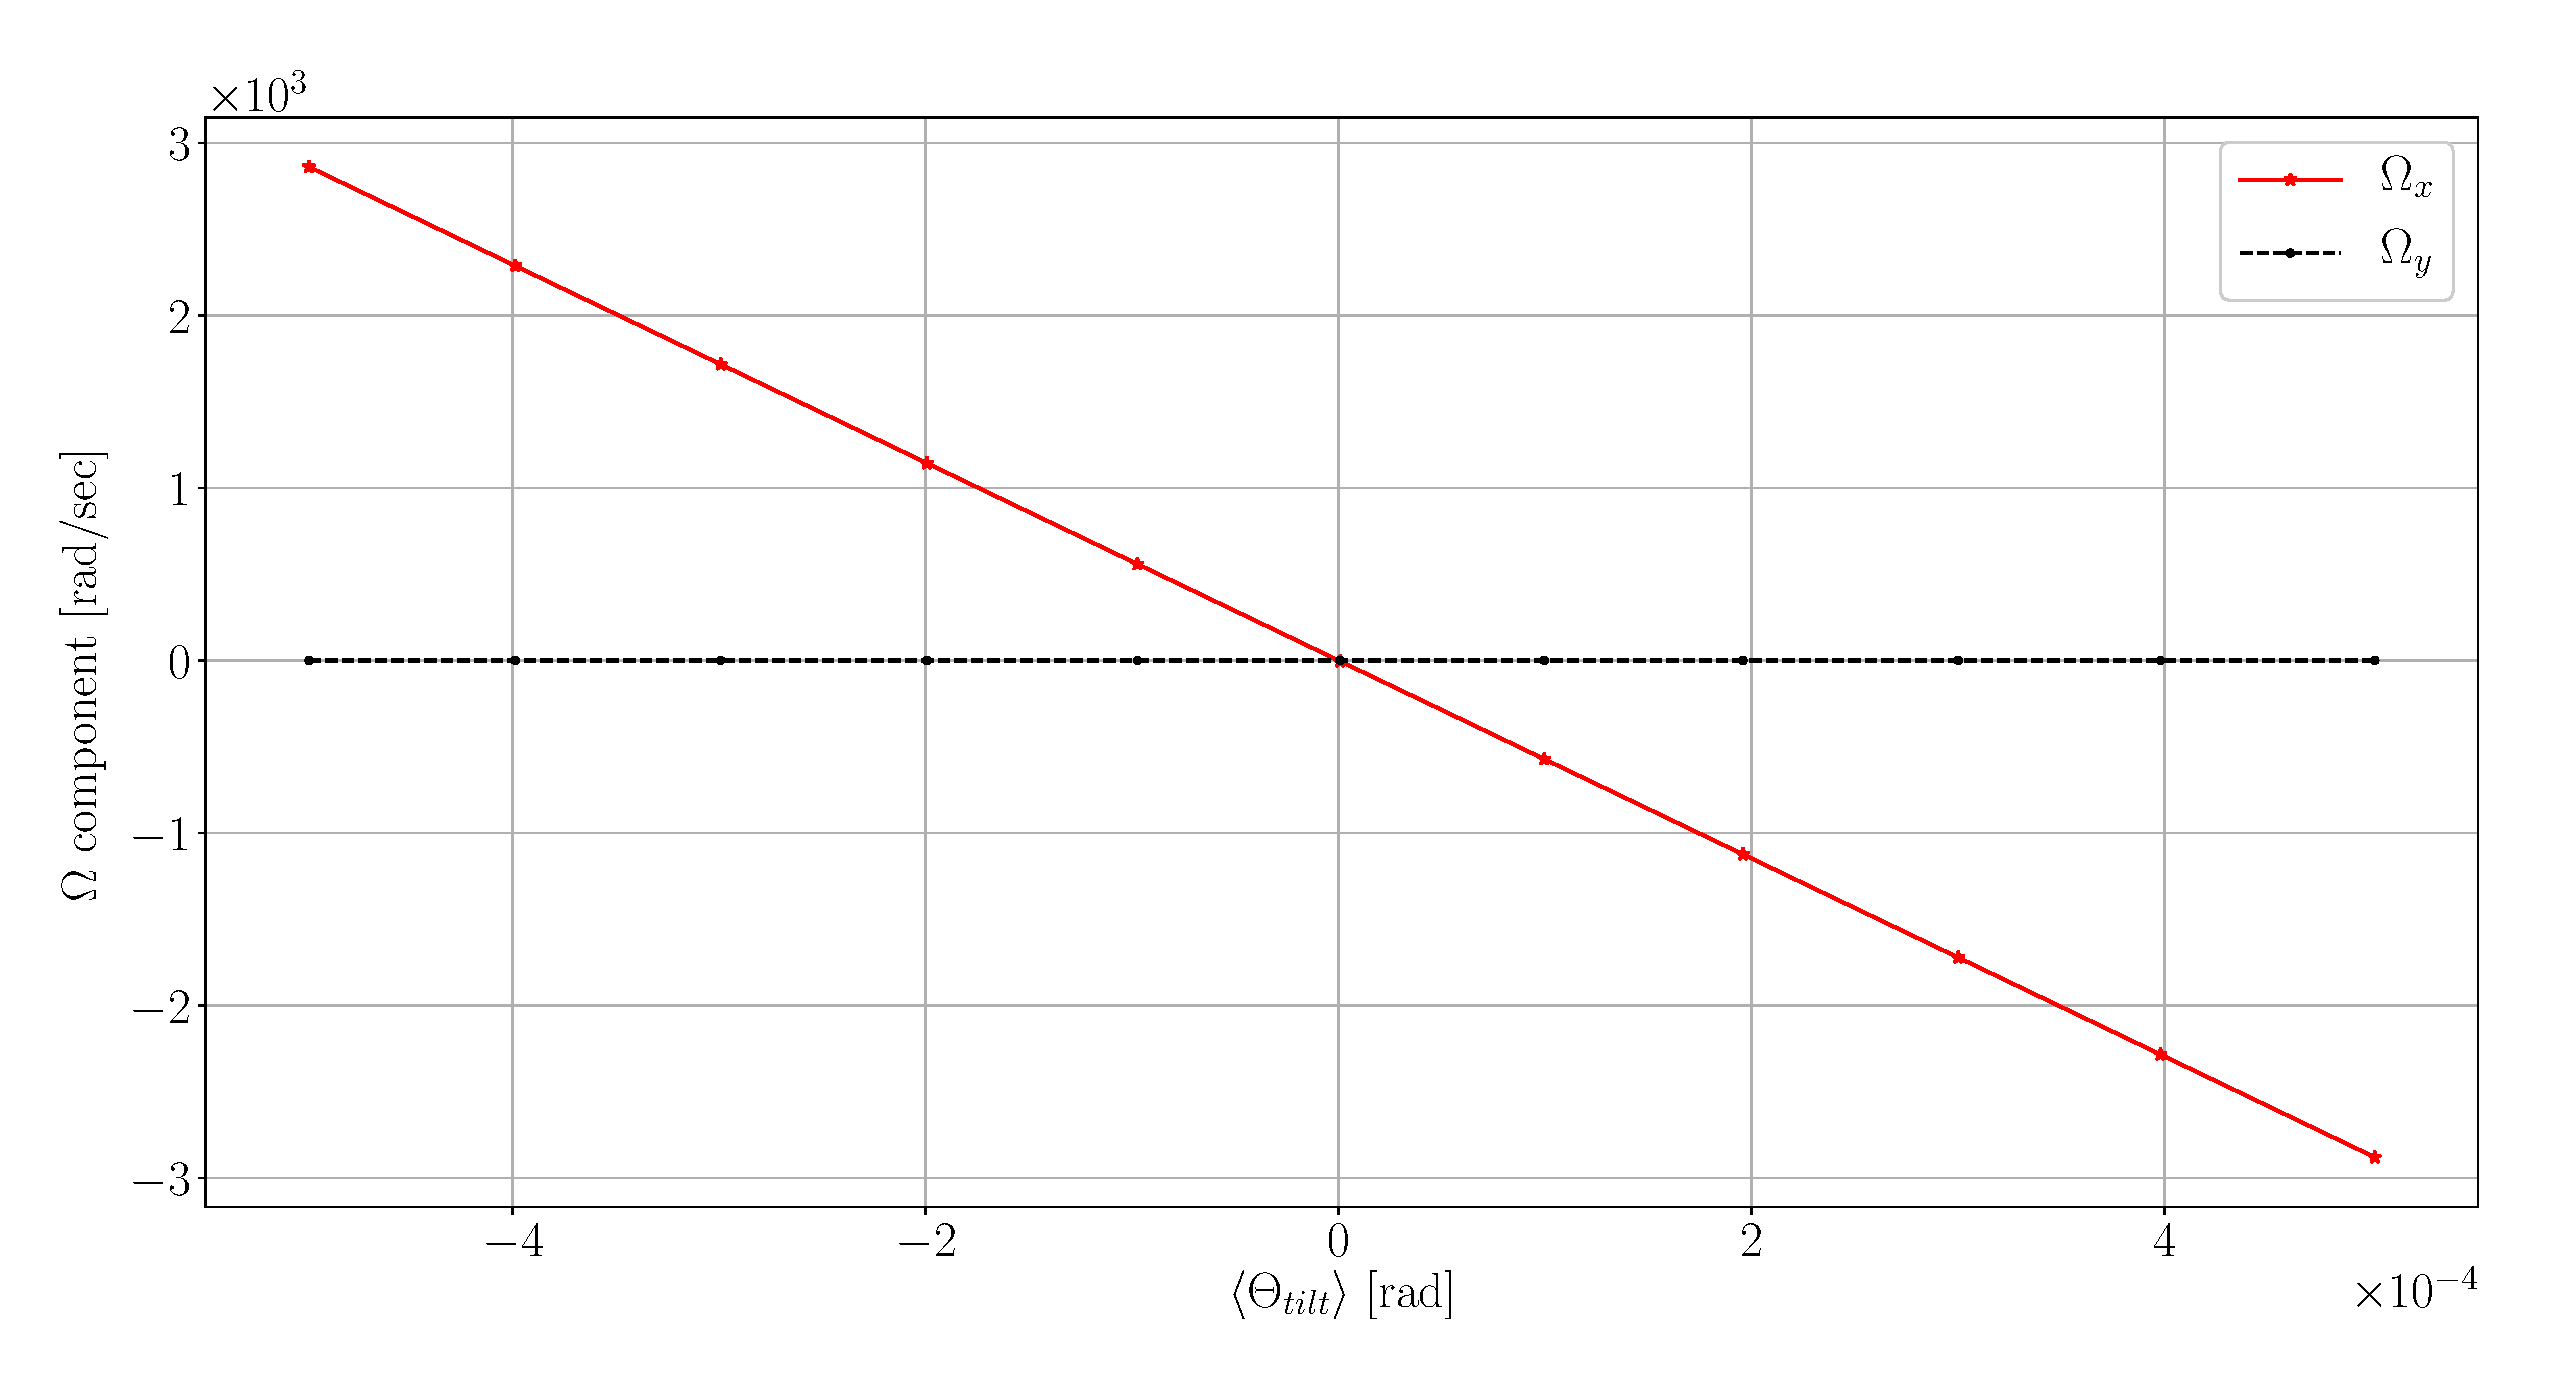
\includegraphics[width=.6\linewidth]{Figures/linearity_test_shifting_gauss_freq}\hspace{3mm}%
	\begin{minipage}{.35\linewidth}\caption{Spin precession angular velocity components vs mean E+B element tilt angle.\label{fig:MDM_vs_tilt}}
	\end{minipage}
\end{figure}

\section{BNL and Koop Method}
The idea of searching for the electric dipole moment (EDM) of the proton and the deuteron using polarized beams in a storage ring is based on the ``frozen'' spin method and was originally proposed at Brookhaven National Laboratory (BNL)~\cite{Farley}.

\begin{equation}\label{eq:Omega}
\Omega=\sqrt{\left(\Omega_{edm}+\Omega_{B_r}\right)^{2}+\Omega_{B_v,E_r}^{2}+\Omega_{B_z}^{2}}	
\end{equation}

\section{Frequency Domain Method}
\subsection{EDM estimator statistic}
Since the measured angular velocity $\W = \W_{MDM} + \W_{EDM}$ includes a contribution due to the MDM, one has to find a way to eliminate the $\W_{MDM}$ term from the final $\hat\W_{EDM}$ estimator. 

In the proposed methodology, non-spurious $\W_{MDM}$ is generated only by the radial magnetic fields induced by accelerator element tilts about the optical axis. Therefore, by reversing the polarity of the guide field one also reverses the sign of $\W_{MDM}$. The EDM estimator is constructed as a sum of positive (beam circulates clockwise) and negative (counter-clockwise) polarity cycles' angular momentum estimates:
\begin{align}
\W^{\pm} &= \pm \W_{MDM}^\pm + \W_{EDM},\\
\hat\W_{EDM} &= \frac12\left[\hat\W^+ + \hat\W^-\right] \notag\\
&= \W_{EDM} + \frac{1}{\sqrt{2}}\cdot\sigma_{MDM} + \epsilon,	\label{eq:EDM-estimator}
\end{align}
where
$\sigma_{MDM}$ is  the statistical (model parameter estimate) error, and the difference between the two cycles' MDM spin precession rates $\epsilon~=~\frac12\left(\W_{MDM}^+~-~\W_{MDM}^-\right)$ is the  systematic error term.

\subsection{Effective Lorentz factor}
In order to minimize systematic error $\epsilon$, one needs a way to keep $\W_{MDM}$ constant across multiple runs.

The obvious way of trying to precisely reproduce the guiding field is inefficient for two major reasons:
\begin{enumerate*}[(1)]
	\item standard magnetic field measurement methods do not yield sufficient precision;
	\item the lattice might not be symmetric enough, in terms of spin dynamics, with respect to reversal of the beam circulation direction.
\end{enumerate*}
Hence, we propose a different variable for calibration.

We note that the number of spin revolutions per turn (spin tune $\nu_s$) depends on the particle's  equilibrium-level energy, expressed by the Lorentz factor $\gamma$:
\begin{align}\label{eq:spin_tune_vs_gamma}
\nu_s^B &= G\gamma, \tag{magnetic field}\\
\nu_s^E &= \frac{G+1}{\gamma} - G\gamma. \tag{electric field}
\end{align}

Not all beam particles in a bunch are characterized by the same $\gamma$. A particle involved in betatron
motion will have a longer orbit, and as a direct consequence of the phase stability principle,
in an accelerating structure utilizing an RF cavity, its equilibrium energy level 
must increase.

The effective Lorentz factor is a generalization of the regular Lorentz factor accounting for betatron motion-related orbit lengthening and non-linearity of the momentum compaction factor.

It has been shown in~\cite[p.~56]{Aksentev:Thesis} that a particle's spin tune can be described by a univariate function; we associate the argument of that function with the effective Lorentz factor. Consequently, spin-vectors of two particles characterized by the same value of the effective Lorentz factor precess as the same rate.

Therefore, if the CW and CCW beam centroids' have equal $\geff$, we can expect the MDM components of the spin precession angular velocities to be equal as well.

\subsubsection{Calibration of the ELF}
Calibration of the effective Lorentz factor is done via observing spin precession in the closed orbit plane. For that purpose, a special transverse spin rotator element is used in order to suppress the vertical plane precession.  Using the fact that $\nu_s$ is an injective function of $\geff$, it follows that there exists a unique value $\geff^0$, at which the polarization vector is frozen with respect to the beam's momentum vector in the horizontal plane, i.e. $\nu_s=0$ in the rest frame. Since the tilt of the spin precession axis is the same for the CW and CCW beams,  
\[
\lim_{\nu_s^+ - \nu_s^- \to 0} \W_{MDM}^+ - \W_{MDM}^- = 0,
\]
and hence $\epsilon$ in equation~\eqref{eq:EDM-estimator} is removed.

\section{Statistical precision}
Spin precession angular velocity is estimated via non-linear fit of a constant-parameter harmonic function to polarization data. However, perturbations to the spin dynamics, caused by, for example, betatron motion, introduce a mismatch between the fit model and the data, and hence a model specification systematic error. This problem has been analyzed,~\cite{Aksentev:IPAC19:SMP} with the conclusion that this systematic error is negligible.

Effective measurement cycle length cannot exceed three times the polarization lifetime $\tau_d$,~\cite{Stats} where $\tau_d$ is the time during which beam polarization decreases by a factor of $e$.

Simulation shows~\cite{Stats} the possibility of reaching a statistical error $\sigma[\hat\W]~=~8\cdot~10^{-7}$~rad/sec in one measurement cycle (at $\tau_d = 721$~sec, cycle length $10^3$~sec), and $\sigma[\avg{\hat\W}]~=~5\cdot~10^{-9}$~rad/sec in one year of measurement (at 70\% accelerator time load). This should suffice to achieve an EDM estimate precision level of $10^{-29}~e\cdot$cm.

\section*{References}
\begin{thebibliography}{4}
	\bibitem{Senichev:FDM}
	Senichev Y, Aksentev A, Ivanov A and Valetov E  2017 Frequency domain method of the search for
	the deuteron electric dipole moment in a storage ring with imperfections, \textit{Preprint} arxiv:1711.06512 [physics.acc-ph]
%	\url{https://arxiv.org/abs/1711.06512}.
	\bibitem{Aksentev:Thesis}
	Aksentev A 2019 2D Frozen spin method of searching for the deuteron EDM in a storage ring \textit{Preprint} thesiscommons.org/cn4x3
%	\url{http://collaborations.fz-juelich.de/ikp/jedi/public_files/theses/dissertation.pdf}
	\bibitem{Aksentev:IPAC19:SMP}
	Aksentev A, Senichev Y 2019 Spin Motion Perturbation Effect on the EDM Statistic
	in the Frequency Domain Method \textit{Proc. 10th International Particle Accelerator Conference (IPAC'19)} 19--24 May 2019 Melbourne, Australia pp 861--863
%	\url{https://ipac2019.vrws.de/papers/mopts011.pdf}
	\bibitem{Stats}
	Aksentev A E, Senichev Y V 2017 Statistical precision in charged particle EDM search in storage rings \textit{J Phys: Conf Ser.} \textbf{941} 012083
%	\url{https://iopscience.iop.org/article/10.1088/1742-6596/941/1/012083}
	
\end{thebibliography}

\end{document}